\documentclass[10pt]{article}
\usepackage{cite}
\usepackage{fancyhdr}
\usepackage[svgnames]{xcolor}
\usepackage{url}
\usepackage{tikz}
\usetikzlibrary{shapes,snakes,arrows}
\usepackage{hyperref}
\usepackage{graphicx}
\usepackage{caption}
\usepackage{subcaption}

\topmargin=-5mm
\evensidemargin=0cm
\oddsidemargin=0cm
\textwidth=16cm
\textheight=22cm
\addtolength{\headheight}{1.6pt}
\hypersetup{pdfstartview=}

\tikzset{>=latex}

\newcommand{\secref}[1]{\S\ref{#1}}

\newcommand{\lastupdate}{\today}
\newcommand{\ie}{\textit{i.e.}}
\newcommand{\mdash}{---}
\newcommand{\ecall}{\textsf{ecall}}
\newcommand{\ocall}{\textsf{ocall}}
\newcommand{\env}{\textsf{environment}}
\newcommand{\mrenclave}{\textsf{mrenclave}}
\newcommand{\mrsigner}{\textsf{mrsigner}}
\newcommand{\sha}{\textsf{sha256}}
\newcommand{\pve}{\textsf{PvE}}
\newcommand{\pce}{\textsf{PcE}}
\newcommand{\qe}{\textsf{QE}}
\newcommand{\launchenclave}{\textsf{Launch Enclave}}
\newcommand{\uc}{\textsf{UC}}

\title{\bf A framework for analyzing Intel SGX Enclaves}
\author{\textsc{Yogesh Prem Swami}}

\date{\lastupdate}

\begin{document}
\pagenumbering{arabic}

\maketitle

\begin{abstract}
  Intel SGX enclaves provide hardware enforced confidentiality and
  integrity guarantees for running pure computations (\ie, OS-level
  side-effect-free code) in the cloud environment. In addition, SGX
  remote attestation enables enclaves to prove that a claimed enclave
  is indeed running inside a genuine SGX hardware and not some
  (adversary controlled) SGX simulator.

  Since cryptographic protocols do not compose well
  \cite{ucframework}, especially when run concurrently, SGX remote
  attestation is only a necessary pre-condition for securely
  instantiating an enclave. In practice, one needs to analyze all the
  different interacting enclaves as a single protocol and make sure
  that no sub-computation of the protocol can be simulated outside of
  the enclave. In this paper, we present a practical framework for
  analyzing enclaves. We analyze Intel provided EPID\cite{epid}
  \textsf{Provisioning} and \textsf{Quoting} Enclave\cite{sgxattest}
  within this framework and report our (largely positive) findings. We
  also provide details about SGX's use of EPID and report (largely
  negative) results about claimed anonymity guarantees.

\end{abstract}

\section{Introduction}
\label{sec:intro}
  Intel SGX enclaves\cite{sgxinnov, sgxinnov2} provide hardware
  enforced confidentiality and integrity guarantees for running pure
  computation (\textit{i.e.}, OS-level side-effect-free code) in the
  cloud environment. By limiting the application's Trusted Computing
  Base (TCB) to the CPU and CPU-Cache, SGX provides unprecidented
  confidentiality and integrity guarantees against malicious OS
  kernels and supervisor software. A popular design methodology---as
  evidenced by \cite{Haven, Graphene, Scone}---for creating secure
  cloud applications is as follows:

  \begin{description}
    \item[Step-1:] First, define a remote-attestation mechanism to
      securely instantiate an enclave. Quite often, this step is not
      explicitly stated probably because a generic black-box
      attestation scheme---whatever that means---is expected to be
      sufficient.
    \item[Step-2:] Then, largely independently of the
      remote-attestation mechanism, define the functionlity that needs
      to be implemented inside the enclave. This step often involves
      composing different cryptographic as well as non-cryptographic
      protocols in ad-hoc ways to implement the desired algorithm. For
      example, the enclave may need to read encypted keys from disk,
      compute a signature based on that key, create a new set of keys,
      etc.
    \item[Step-3:] Finally, define a ``run-time workflow," where one
      first validates the remote-attestation result, and then runs the
      algorithm implemented by the enclave. This step often requires
      multiple interactions with various other entities such as other
      enclaves, untrusted host software, trusted remote client
      softrware, and other cryptographic devices such as TPMs.
  \end{description}

  It's hard to argue against the simplicity and ease of implementation
  of such a modular software design. However, as pointed out in
  \cite{ucframework}, unless a protocol is desgined for
  ``\textsf{Universal Composition}" (\uc)---where, the real-world
  behavior and the ideal-world definition (function) of a protocol are
  computationally indistinguishable \textit{for every} adversary
  controlled environment---it's unlikely that arbitrary composition of
  such protocols will be secure. On the other hand, proving results in
  the \uc-framework is rather difficult. In this paper we propose a
  framework for analyzing SGX enclaves that's a compromize between a
  full \uc-based analysis and completely ad-hoc composition. Before
  describing the framework, we illustrate the problem associated with
  the protocol composition with two real-world examples.

  To set the stage, a cloud service provider\footnote{This example is
    based on a distilled version of actual protocol designed by a
    mid-sized cloud-security/compliance company.} wanted to migrate
  its new clients from Amazon Cloud-HSM to an SGX enclave. The
  protocol for interacting with the enclave was based on HTTP
  Request/Response framework, where different operations (such as
  \textsf{KeyGen}), were sent as a command, and the enclave would
  execute and return a response (including explicit error codes) back
  to the remote caller.  Important use-case for the enclave were to
  support (a) local key generation, (b) storing the public/private key
  on disk with an AEAD scheme that would allow \textit{fast}
  key-lookup, and (c) creating Certificate Signing Requests (CSR) from
  the enclave using challenge-response protocol
  \cite[\S5.2.8.3]{rfc4210}, among other
  things. Figure~\ref{fig:sequentialcomp} describes one execution path
  of the protocol.

  \begin{figure}[h]
  \centering
  \begin{subfigure}[b]{.5\textwidth}
    \centering
    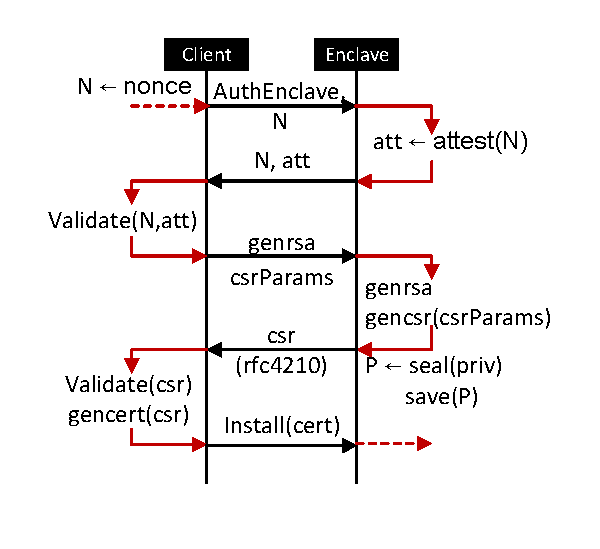
\includegraphics[width=.95\linewidth]{Diagrams/SeqCompProblem}
    \caption{Command execution for \textsf{KeyGen} with Cert}
    \label{fig:sequentialcomp}
  \end{subfigure}%
  \begin{subfigure}[b]{.5\textwidth}
    \centering
    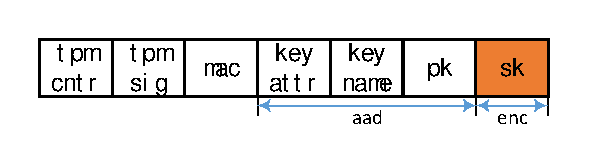
\includegraphics[width=.95\linewidth]{Diagrams/MsgFmt}\\\vfill
    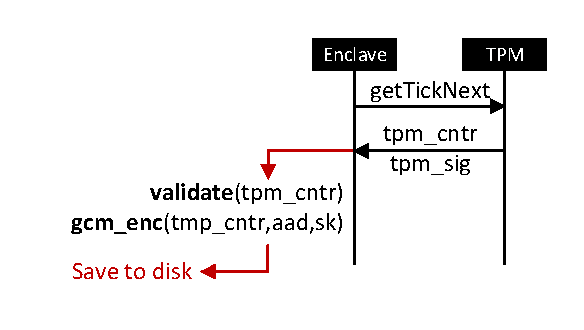
\includegraphics[width=.95\linewidth]{Diagrams/SealProtocol}
    \caption{Message format and seal protocol}
    \label{fig:sealprotocol}
  \end{subfigure}
  \caption{Example of a flawed key-management enclave. The commmand
    execution protocol ascertains the authenticity of the enclave by
    validating the EPID signature on a randomly generated 256-bit
    nonce, followed by executing an arbitrary mix of commands as
    required by the use-case. Long-term keys are stored as
    GCM-encrypted AEAD blobs. The nonce (a 32-bit counter zero-padded
    on the left to 96-bit) for each GCM record is stored in TPM, and
    the TPM returns a signature on the nonce (along with some
    additional data---to disable roll-back of TPM ``ticks.'' The
    enclave validates the TPM's signature before using the nonce for
    sealing.}
  \label{fig:usecase}
  \end{figure}

  This seemingly secure protocol is however not secure at all. Notice
  that the remote attestation in Figure~\ref{fig:sequentialcomp} does
  not prevent a malicious cloud service provider from first faithfully
  responding to remote attestation queries, but then emulate the rest
  of the protocol (including \textsf{KeyGen} and CSR) outside of the
  enclave. While this is obvious in this simplified example, in a more
  complicated scanerio, where multiple enclaves are interacting with
  each other, it might not be obvious if certain subcomponents of the
  protocol can be simulated outside. Even though the entire enclave is
  \textit{sequentially composed} from potentially provably-secure
  protocols, the combined protocol is completely insecure.

  Second, consider the seal protocol. Here each record (see
  Figure~\ref{fig:sealprotocol}) is GCM-encrypted using a nonce
  generated and signed by a TPM. However, consider a cloud service
  provider who instantiates two copies of the same enclave and
  \textit{concurrently} executes \textsf{KeyGen} using the same TPM
  signed counter. In this case, each enclave will generate two
  different keys in response to \textsf{KeyGen}. However, since the
  two concurrent instances will each correctly verify the signature
  (the two enclaves are identical), each will end up using the same
  nonce with different underlying data! As is the case with all
  counter modes, reusing the nonce can completely destroy the security
  of the system\footnote{In the present case, since the underlying
    data is uniformly distributed, at least for AES or ECDSA keys,
    such a concurrent composition might not be harmful. However, if
    there is even a small bias in the random number generator, it
    might be possible to build a distinguisher from the \texttt{xor}
    of plain-text data.}. Note that this is not a flaw in GCM or in
  the way the TPM is used\footnote{When using TPMs with SGX enclaves,
    it's important that both the TPM and the enclave mutually
    authenticate each other. Failure to do so can lead to replay
    attacks where the adversary swaps the motherboard and in doing so
    resets the TPM counter. In the present case, however, even
    mutually authenticated TPM counter might not be secure under
    concurrent composition.}, rather, it's a case where an otherwise
  secure protocol is insecure under concurrent composition.

  To summarize, \textit{an enclave is a protocol} composed of several
  sub-protocols. In order for the enclave to be secure, it's essential
  that sequential and concurrent composition of subprotocols remain
  secure. Here, by secure, it's meant that the internal state of the
  enclave cannot

  The rest of this document is organlized as follows.
  \secref{sec:model} describes the abstract computational model that's
  better suited for security ananysis. \secref{sec:analysisfwk}
  describes pitfalls of sequential, concurrent, and parallel
  composition of cryptographic protocols and describes ways in which
  an enclave can be abused by a malicious cloud service
  provider. \ref{sec:remoteatt} describes Intel's remote attestation
  framework, and describes in detail the SGX remote attestation
  mechanism.

  \section{SGX Computational Model}
  \label{sec:model}
  Intel documentation\cite{intelsdm} provides excellent low-level
  details about the SGX instructions. This section provides an
  abstract computational model of SGX which is better suited for
  security analysis of an SGX enclave.

  Abstractly, an SGX enclave can be thought of as a blackbox that's
  capable of running any arbitrary algorthim. The blackbox, hereafter
  called an enclave, communicates with the outside world, called the
  \env, in three different ways:

  \begin{figure}[h]
  \centering
  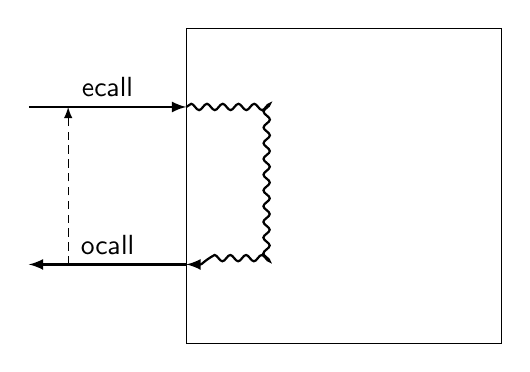
\begin{tikzpicture}[x=1cm, y=-1cm]
  \newcommand{\ench}{4cm}
  \newcommand{\encw}{4cm}
  \newcommand{\alen}{1cm}
  \newcommand{\adiff}{1cm}

  \node[rectangle, minimum height=\ench, minimum width=\encw, draw] (enc) {};
  \draw[->,thick] (-\encw / 2.0 - 2*\alen, \adiff ) -- (-\encw/2.0, \adiff) %%
  node [midway, above] {\textsf{ecall}};

  \draw [->, thick, decorate, %%
    decoration={snake,amplitude=.4mm,segment length=2mm, post length=1mm}] %%
  (-\encw/2.0, \adiff) -- (-\encw/2.0 + 1*\adiff + 0.1, \adiff) -- %%
  (-\encw/2.0 + 1*\adiff , -\adiff) -- (-\encw/2.0, -\adiff);


  \draw[<-,thick] (-\encw / 2.0 - 2*\alen, -\adiff ) -- (-\encw/2.0, -\adiff) %%
  node [midway, above] {\textsf{ocall}};

  \draw[->, thin,densely dashed] (-\encw / 2.0 - 1.5*\alen, -\adiff ) -- %%
  (-\encw/2.0 - 1.5*\alen , \adiff);
\end{tikzpicture}

  \caption{SGX Computational Model.}
  \label{fig:model}
  \end{figure}

  \begin{description}
  \item[Ecall:] The \env\ can invoke a pre-defined function inside the
    enclave by passing input parameters and returning internal state
    of the enclave as results. Such invocations from the \env\ to the
    enclave are referred to as \ecall. The parameter values passed
    from the \env\ to the enclave are either copied or directly shared
    with the enclave. An \ecall\ can terminate in one of the three
    ways: (a) by returning from the enclave, (b) by making an explicit
    \ocall, or (c) as a result of an interrupt or exception.

    SGX also supports multithreading, and it's possible for the
    \env\ to run the same \ecall\ in different threads. However, once
    an \ecall\ has acquired the thread, future attempts to reuse that
    same thread will result in error. Futhermore, the number of
    threads that an enclave can support is pre-determined by the
    enclave signer, and cannot be altered at runtime.

  \item [Ocall:] While an enclave is executing (because of some
    previous \ecall), it can make \ocall s to pre-designated functions
    in the \env.  Unlike an \ecall, an \ocall\ cannot directly share
    the internal enclave state with the \env, and must---directly or
    indirectly---copy the parameters into the \env\ before making an
    \ocall.

    An interesting characteristic of an \ocall\ is that the \env\ is
    not requred to return back to the enclave at the end of the
    \ocall\ (see Figure~\ref{fig:model}). Since the behavior of
    pre-designated functions in the \env\ are controlled by the
    adversary, one should not expect the \env\ to follow the protocol
    that enclave author envisioned. In particular, it's possible to
    create a chain of \ecall s and \ocall s such that the adversary
    can perform operations on the internal (global) state of the
    enclave.

  \item[Asynchrnonous Exit:] In addition to an \ocall, the processor
    can exit from an enclave due to an interrupt or exception. Such
    enclave exiting events are called Asynchronous Exit Events, or
    AEX. Unlike an \ocall, an AEX can transfer control from the enlave
    to the environment at arbitrary (possibly adversary controlled)
    points inside the enclave. Like \ocall s, an AEX can either by
    resumed from where the enclave left off, or the environment can
    invoke another \ecall (either within the same thread or a
    different thread).

    Since an adversary can create multiple running copies of an
    enclave and selectively interrupt each enclave to cause and AEX,
    it can be used as a means to ``rewind'' the internal state of of
    the enclave. Given that proof-of-knowledge \cite{BellarePOK}
    protocols fundamentally have a \textit{knowledge-extractor} based
    on rewinding, an enclave must ensure that it does not leak secrets
    when interrupted by an AEX.

  \end{description}

  \subsection{Enclave Creation}
  \label{sec:enclavecreateion}
  An enclave is generated as a dynamically shared library using
  standard compiler tools. In addition, the entity creating the
  enclave must also decide up-front on the following information:

  \begin{description}
  \item[Attributes]: The attributes of an enclave act as an access
    control mechanism that is enforced by the hardware. For example,
    certain high priviledge keys, such as Launch-Key and Provision-Key
    cannot be made accessible to all the enclaves, as it would
    compromize the security of entire SGX ecosystem---not just a given
    CPU. An enclave author requests the attributes needed by the
    enclave at compiler/sign time, and the Launch-Enclave, based on
    policy decisions, decides whether to grant or reject an
    authorization token (called \textsf{EINITTOKEN}) for instantiating
    the enclave.

  \item[Stack size]: The enclave author must estimate the size of the
    stack needed by enclave and set its value at enclave creation
    time.  Once an enclave is instantiated, this value cannot be
    changed.

  \item[Heap size]: Like the stack size, the heap-size of the enclave
    is also fixed at enclave creation time. In SGXv2, this value can
    be changed post instantiation.

  \item[Thread count]: An enclave must also decide upon the number of
    threads that can run conconrrently. As pointed out in
    \secref{sec:model}, concurrency can have a dramatically negative
    impact on the security of the certain protocols, and one must not
    select this parameter just on the basis of performance
    requirements, but also on the basis of security concerns.

  \item[Software versioning]: SGX provides elaborate software-upgrade
    and life-cycle management faciliaties and allows software vendors
    to make use of these features.
  \end{description}

  Based on these parameters, the enclave signing tool creates a
  virtual memory layout of the enclave and comptes a hash of the
  entire memory layout (including the stack, heap, thread control
  structure, etc.)  See \cite{intelsdm} for details about how the hash
  is computed. This hash, called \mrenclave, is used as the unique
  identifier for the enclave.

  In addition to \textsf{mrenclave}, the software vendor must also
  sign the enclave using a RSA-3072 key. The hash of the RSA
  Public-Key is called \mrsigner. As described in \cite{surnaming},
  the purpose of the signature is to provide an unforgeable
  identity---a \textit{surname} based lineage---to a set of enclaves
  based on the vendor.

  It should be noted that the \mrenclave\ of an enclave doesn't
  change even when the signing key is changed. This is significant
  when validating attestation or deriving keys based on \mrenclave.

  \subsection{Enclave Instantiation and Access Control}

  A properly signed enclave can be instantiated on any Intel SGX
  Processor---subject to access control restrictions enforced by
  \launchenclave. Before an enclave can be instantiated on an SGX
  capable processor, it must get an authorization token, called
  \textit{Launch Token}, from Intel provided \launchenclave. The
  \launchenclave\ uses a combination of \mrenclave, \mrsigner, the
  attributes of the enclave and a \textit{whitelist signed by Intel}
  to decide whether to grant Launch Token to the enclave or not. Once
  an enclave obtains a Launch Token, the enclave can continue using it
  indefinitely, even when the policies of the \launchenclave\ might
  get updated later on.

  \subsection{SGX Platform Keys}

  As described in \cite{sgxattest}, each Intel SGX capable processor
  contains two statistically independent base keys: \textit{Root
    Provisioning Key} and \textit{Root Seal Key}. The Root
  Provisioning Key is used as the Root of trust between the CPU and
  Intel Attestation Services (IAS) \cite{ias}. Intel retains a copy of
  this key at the time of manufacturing and uses it to establish the
  trustworthiness of the processor during EPID join process. Intel
  claims that Root Seal Key is not retained. However, it's not clear
  whether the this key is generated inside the processor via oracle
  access (\ie, in such a way that CPU generates the key all by itself
  using it's own internal random numbers or with PUFs), or whether the
  key is first generated outside the processor, then injected into
  CPU, and finally all outside references destroyed. Unless these keys
  are generated via oracle access, one should consider the Root Seal
  Key to be known to Intel.

  \begin{figure}[h]
  \centering
  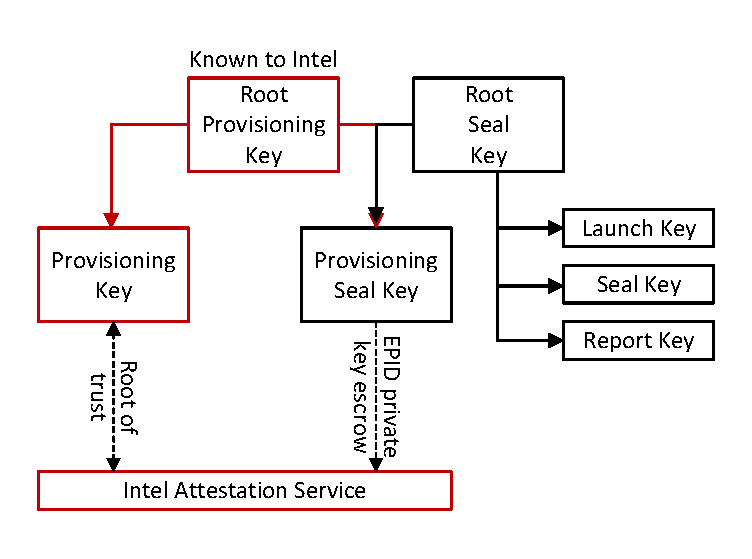
\includegraphics[scale=.75]{Diagrams/KeyHierarchy}
  \caption{Intel SGX Platform Keys}
  \label{fig:keys}
  \end{figure}

  An application software does not have raw acceess to these base
  keys. However, an application can access following \textit{named}
  keys that are derived from these two base key (see
  Figure~\ref{fig:keys}):

  \begin{description}
  \item[Provisioning Key]: This key is derived from Provisioning Key
    and is used as the root-of-trust between the CPU and the Intel
    Attestation Service during the EPID join process. Since admitting
    a non-SGX processor to the Intel Attesttion Service's group of SGX
    Processors will completely compromize Remote Attestation of all
    CPUs, extreme care must be taken in granting access to
    Provisioning Key.  Currently, the \launchenclave\ only grants
    Provisioning Key access to enclaves that have been signed by
    Intel. Furthermore, only Provisioning Enclave (\pve) and
    Provisioning Certification Enclave (\pce) (both created without
    debug option) have access to Provisioning Key.


  \item[Provisioning Seal Key]: This key is derived joinly from Root
    Provisioning Key and Root Seal Key. The EPID join process, the
    EPID private-key for each platform is encrypted with this key and
    uploaded to Intel Attestation Service. (See \secref{ssec:epidprov}
    for details about EPID join process.)

    Note that the EPID private-key could not just be encrypted with
    Provisioning Key as that would destory the EPID's blinded-join
    protocol. Conversely, the EPID private-key cannot be encrypted
    just with Seal Key as that might allow non-priviledged enclaves to
    have access to EPID private key and thereby render Remote
    Attestation ineffective\footnote{If someone could access EPID
      private key---either directly, or through oracle access---they
      could sign remote attestation queries for \textit{any}
      platform. Furthermore, because of anonymimity, it will be
      difficult to determine the platform that was compromized.}.

    In spite of this design choice, given the uncertainity about how
    the Root Seal Key is generated, one should assume that Intel knows
    the EPID private key for each platform.

  \item[Launch Key]: This key is derived from Root Seal Key and is
    used by \launchenclave\ to create authorization tokens
    (\textsf{EINITTOKEN}) that each non-Intel enclave must obtain in
    order to instantiate an enclave. Only a specific \mrsigner---whose
    corresponding private-keys are only known to Intel---can access
    the Launch Key. In SGXv2, the \mrsigner\ for \launchenclave\ can
    be changed programatically, (see \cite[\S39.1.4]{intelsdm} for
    details) and any enclave signed with that \mrsigner\ can gain
    access. With this change, however, it's not clear how Intel
    intends to enforce access control restrictions on the
    Proviosioning Key.

  \item[Seal Key]: This key is derived from Root Seal Key and used
    for encrypting data specifically for a given CPU.

  \item[Report Key]: This key is derived from Root Seal Key and used
    for Local Attestation (see \secref{sec:localatt} for detailed
    information on Local Attestation how Report Key is used).
  \end{description}

  In addition to the named keys, each key can be further diversified
  using a 128-bit user selected constant called \textit{Key Wearout
    Protection}.  In addition, certain keys can be further diversified
  using \mrenclave\ or \mrsigner\ of the enclave.

  \subsection{Local Attestation}
  \label{ssec:localatt}

  \section{Framework for Analyzing SGX Enclave}
  \label{sec:analysisfwk}

  While an SGX enclave is generally presented as a programming tool to
  conceal the computational state of an algorithm, in practice each
  enclave implements a protocol between the \env\ and the algorithm
  that the enclave implements. The \ocall s, \ecall s, and AEX define
  the external interface for interacting with the protocol. An enclave
  can be considered secure only if the \textit{overall protocol}
  implemented by the enclave is secure.

  As described in \secref{sec:intro}, sequential, concurrent, and
  parallel composition of otherwise secure protocols, does not
  necessarily result in an overall secure system. One way to formalize
  the overall security of an enclave would be consider the

  \subsection{Concurrent Enclave Execution}
  \label{ssec:concexec}

  \subsection{Parallel Enclave Execution}
  \label{ssec:parallelexec}

  \subsection{Enclave Rewinding}
  \label{ssec:rewinding}

  \section{SGX Remote Attestation}
  \label{sec:remoteatt}

  \subsection{EPID Overview}
  \label{ssec:epid}

  \subsection{SGX Pairing Groups}
  \label{ssec:pairings}

  \subsection{SGX EPID provisioning}
  \label{ssec:epidprov}

  \subsection{SGX Quoting Enclave}
  \label{ssec:qe}

  \section{Conclusion}
  \label{sec:conclusion}

\bibliographystyle{alpha}
\bibliography{sgx_biblio}

\end{document}
